
\section{Context-free grammars}


Now that we have seen a grammar given by production rules we can explain 
in what way context-free grammars are ``context-free'', and how they 
come to parse as trees.  Consider the situation discussing square-roots 
of natural numbers.
\begin{center}
\begin{gcode}[]
+<Root> ::= + sqrt(<Nat>)
-<Root> ::= - sqrt(<Nat>)
\end{gcode}
\end{center}
In this case \code{sqrt{2}:<Root>}.  However, we do not know if this 
was meant as the positive or negative root.  That information 
was left to the surrounding context in which the term was parsed.  
This is a very useful situation as often in algebra we do want to 
speak within a context.  Yet because of the ambiguity if we 
introduce a root in this way and then seek to eliminate we 
cannot be certain of many possible paths got us here.

Meanwhile 
to make this context-free grammar we could use 
\begin{center}
\begin{gcode}[]
<Root> ::= + sqrt(<Nat>)
         | - sqrt(<Nat>)
\end{gcode}
\end{center}
Now \code{+sqrt(2):<Root>} and \code{-sqrt(2):<Root>} but 
this grammar rejects \code{sqrt(2)}.  The grammar is less forgiving 
but more precise in the content it now holds for us.

\begin{definition}
    A \emph{context-free grammar} is a grammar whose non-constant 
    production rules are defined on their to the left of the astonished Walrus 
    \code{::=}.
\end{definition}

For example, productions rules that begin in the form \code{<Thing>::=...}
are all that we permit.

\begin{definition}
    The \emph{parse-graph} of an accepted string $\sigma$ is 
    defined recursively as the having vertices any production rule 
    which ends in a terminal equal ot $\sigma$, or 
    if $\sigma$ is non-terminal, then vertex for each production rule 
    that accepts $\sigma$ with an edge to any production rules traversed
    by that acceptance.
\end{definition}

\begin{proposition}
    The parse graph of an accepted string of an unambigiuous context free grammar 
    is a unique vertex-labeled tree, with each label a production rule and each leaf 
    an atom (constant/variable symbol).
\end{proposition}
\begin{proof}
    Suppose $x$ is accepted as $x:Token$.  
    Because the grammar is an unambigious grammar 
    it has a unique token that accepts $x$.
    As it is context-free we are guaranteed 
    that $x$ was accepted by a production rule of form 
    \code{<Token>::= A1 ... An} where the 
    \code{Ai}'s are 
    terminal or production rules.  By recursion assign 
    to each \code{Ai} its associated parse graph which
     by induction makes each into a rooted tree.
\end{proof}

A further property that we often exploit but we shall not prove here is that 
context-free grammars are economical to parse.  In fact they do not even 
require the full strength of a computer but could be done with the type 
of system needed to program a microwave.  While Moore's law drove the creation 
of full strength (Turing Complete) microprocessors, the need to reduce energy 
and cost of production has brought a resurgence of such limited ability 
hardware.  
\begin{proposition}
    A context free grammar can be parsed by an automata with a push-down (last-in-first-out)
    stack.
\end{proposition}

For comparison, to parse context-sensitive grammars we suddenly require more 
than Turing machine, we need a nondeterminisitc machine.  That is, we have to make 
some (possibly random) choices about what way to parse.

\subsection{$\mathbb{N}$ as an algebra}
Although we have come to know $\mathbb{N}$ for its addition take note that 
the real work was done by the successor.  In fact the introductions themselves 
point the way to the founding operations of natural numbers.
\begin{enumerate}
    \item The $0$ operator converts nothing into a starting point.  
    \item The successor operator \code{S<Nat>}, abbreviated now to just 
    $S\Box$, converts a given natural number into a new one.
\end{enumerate}

Addition is different from $S$ because addition is not making new 
numbers, it is actually just refashioning numbers into others.  


\begin{remark}
    Many argue that natural numbers should not contain $0$ because we start counting 
    at $1$.  Others argue that because of natural numbers have a place to start 
    and call it what you like the starting place always behave like $0$ when we add.

    Both perspectives have a point but both traffic in a misrepresentation of the 
    situation.  To say that there is a place to start, call it 0, is to say 
    you can begin a tally.  But the act of counting is to tally, that is, the case 
    of $+$, resp. \code{S}. So from $0$ our first count is $1\defeq S(0)$. 
    
    So it transpires that the
    natural numbers do include $0$ (an empty tally board), but at the same time
    we begin counting at $1$.  Neither point of view is possible without the other
    being true.
\end{remark}


\subsection{No relations matter}

One might argue that this is different tally we all use.  For example, in a tally we might 
add strokes to either side.  For instance:
\begin{center}
    \StrokeOne~\StrokeTwo = \StrokeThree = \StrokeTwo~\StrokeOne,
    i.e.\ $1+2=3=2+1$.
\end{center}
This is possible but requires a different grammar.  To make the point clear let us 
use $L$ for tallies on the left and $R$ for tallies on the right.
\begin{center}
\begin{gcode}[]
<LRNat> ::= 0 
         | L <LRNat>
         | <LRNat> R
\end{gcode}
\end{center}
We see this grammar accepts
\begin{center}
    \code{L0:LRNat}, \code{0R:LRNat}, and \code{L0R:LRNat}.
\end{center}
Yet nothing in this treats \code{L0}=\code{0R}.  So this is not quite what we 
want.  Later we shall add relations to the grammar to accomplish that goal.
    

    
\subsection{Formal definitions}

\section{Introducing strings}
The point of basic patterns is to use them in more complex systems
with an understanding of the resulting behavior.  Imagine a string 
of characters in an alphabet a, b, and c.  The grammar evolved to 
have more constants 
\begin{center}
\begin{gcode}[]
<abc> ::=  
       | a <abc> 
       | b <abc>
       | c <abc> 
\end{gcode}
\end{center}
So this grammar accepts \emph{aabaabcac} 
but would reject \emph{adabb} since `d' is not in the list of productions 
rules.  This grammar also accepts an empty string, often denoted 
$\epsilon$.  We can draw the accepted words as a graph with each vertex 
being an already accepted word and an arrow indicated which production rule 
advanced it to another accepted rule.  This builds out an infinite 
3-regular tree, of which we show just a snippet.
\begin{center}
    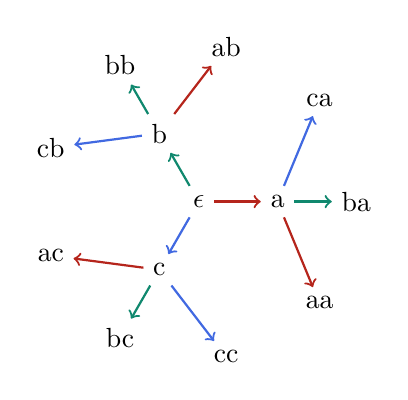
\begin{tikzpicture}
        \node (e) at (0,0) {$\epsilon$};
        \node (a) at (0:1) {a};
        \node (b) at (120:1) {b};
        \node (c) at (240:1) {c};
        \node (aa) at (-40:2) {aa};
        \node (ba) at (0:2) {ba};
        \node (ca) at (40:2) {ca};
        \node (ab) at (80:2) {ab};
        \node (bb) at (120:2) {bb};
        \node (cb) at (160:2) {cb};
        \node (ac) at (200:2) {ac};
        \node (bc) at (240:2) {bc};
        \node (cc) at (280:2) {cc};
    
        \draw[thick,->,BrickRed] (e) -- (a);
        \draw[thick,->,PineGreen] (e) -- (b);
        \draw[thick,->,RoyalBlue] (e) -- (c);
    
        \draw[thick,->,BrickRed] (a) -- (aa);
        \draw[thick,->,PineGreen] (a) -- (ba);
        \draw[thick,->,RoyalBlue] (a) -- (ca);
    
        \draw[thick,->,BrickRed] (b) -- (ab);
        \draw[thick,->,PineGreen] (b) -- (bb);
        \draw[thick,->,RoyalBlue] (b) -- (cb);
    
        \draw[thick,->,BrickRed] (c) -- (ac);
        \draw[thick,->,PineGreen] (c) -- (bc);
        \draw[thick,->,RoyalBlue] (c) -- (cc);
    \end{tikzpicture}
\end{center}
This is another algebra, with one nullary operator 
$\epsilon$ and three unary operators {\color{BrickRed}a$\Box$}, 
{\color{PineGreen}b$\Box$}, and {\color{RoyalBlue}c$\Box$}
being the production rules, that is the tree colors of arrows.

\code{Char:=['a','b',...,'z']}.
\begin{lstlisting}[language=Hidris]
data String = Empty | Prepend( head:Char, tail:String) 
\end{lstlisting}
Writing \lstinline{head:Char} or \lstinline{tail:String} 
indicates that head must come from the alphabet we chose 
and tail must be some already produced string, possibly empty.
Some readers might relate to a different dialect of 
programming such as the following
\begin{lstlisting}[language=Sava]
class String
    case Empty extends String
    case Prepend( head:Char, tail:String) extends String
sealed
\end{lstlisting}
The head here caries around what we put in the list and the tail 
is what comes next in the list.  Observe the similarities:
\begin{align}
     2 & \defeq S(S(0)) \tag{$\mathbb{N}$}\\
 \text{\lstinline{"me"}} & \defeq \text{\lstinline{Prepend('m',Prepend('e',Empty))}}
\tag{String}
\end{align}
The left-hand sides are merely notation for what the data really is on the right.
Both the successor and the \lstinline{Prepend} are operators that generate 
new values.  So part of algebra is to generate new data; so, it is no wonder 
that it closely connections to computation.

